\documentclass{beamer}
%
% Choose how your presentation looks.
%
% For more themes, color themes and font themes, see:
% http://deic.uab.es/~iblanes/beamer_gallery/index_by_theme.html
%
% to be used by pdfpc: https://pdfpc.github.io/
% guide at https://github.com/pdfpc/pdfpc/releases/latest/download/pdfpc-demo.pdf
%
% command to use for this presentation:
% pdfpc --size=1920:1060 UDEC_federated_EN.pdf
\mode<presentation>
{
  \usetheme{Darmstadt}      % or try Darmstadt, Madrid, Warsaw, ... (default)
  \usecolortheme{crane} % or try albatross, beaver, crane, ... (deafult)
  \usefonttheme{structurebold}  % or try serif, structurebold, ... (deafult)
  \setbeamertemplate{navigation symbols}{}
  \setbeamertemplate{caption}[numbered]
  \setbeameroption{show notes} %un-comment to see the notes
} 

\usepackage[english]{babel}
\usepackage[utf8x]{inputenc}
\usepackage{wrapfig}
\usepackage{multimedia}

\title[Unsupervised Clustering in Federated Learning]{UDEC used in a federated setting}
\author{Lorenzo Sani}
\institute{Università degli Studi di Bologna}
\date{\today}

\begin{document}

\begin{frame}
  \titlepage
\end{frame}

% Uncomment these lines for an automatically generated outline.
%\begin{frame}{Outline}
%  \tableofcontents
%\end{frame}

% \section{Federated Learning (FL)}

% \begin{frame}{Federated Learning (FL) in breve}
% 	Caratteristiche generali:
% 	\cite{9153560}
% 	\cite{mcmahan2017communicationefficient}
% 	\begin{itemize}
% 		\item evitare la necessità di costituire grandi dataset "aggregati"
% 		\item sfruttare le nuove tecniche di deep learning (DL)
% 		\item definire la migliore procedura di aggregazione
% 	\end{itemize}
% 	Vantaggi:
% 	\begin{itemize}
% 		\item quasi nessuna limitazione sui dati dovuta alla privacy
% 		\item migliore sfruttamento delle risorse di calcolo (sale server)
% 		\item il framework Flower è semplice e "modellabile" \cite{beutel2021flower}
% 	\end{itemize}
% 	Svantaggi:
% 	\begin{itemize}
% 		\item i principali algoritmi di aggregazione si adattano bene solo alle reti neurali
% 	\end{itemize}
% \end{frame}

\section{UDEC}

\begin{frame}{Unsupervised Deep Embedding for Clustering (UDEC)}
	Aims:\cite{DBLP:journals/corr/XieGF15}
	\begin{itemize}
		\item learning feature representations of data
		\item learning clustering assignments
	\end{itemize}
	Methods:
	\begin{itemize}
		\item denoising autoencoder
		\item a DNN optimized for the clustering objective
	\end{itemize}
	\centering
	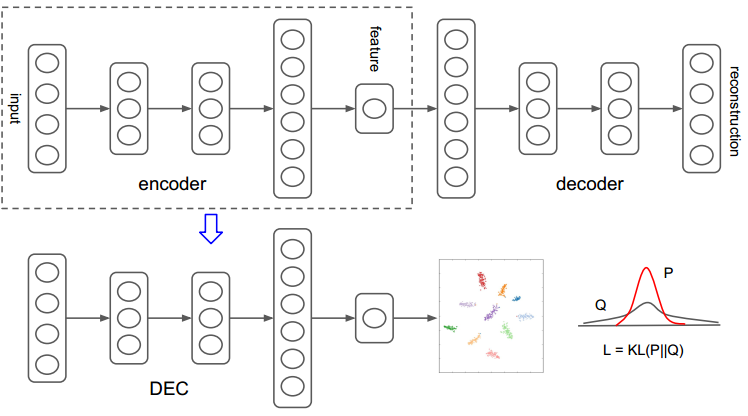
\includegraphics[width=0.6\textwidth, keepaspectratio]{./images/UDE_model.png}
\end{frame}

\begin{frame}{Federated Framework\cite{beutel2021flower}}
	\centering
	
\includegraphics[width=0.2\textwidth, keepaspectratio]{./images/flower-logo.png}
	\begin{itemize}
		\item FLOWER Framework is used for simulating a real federated setting, using FedAvg algorithm
		\item 8 equal clients contribute simultaneously to the training and the evaluation at every step
		\item clients are not able to see other clients' data
		\item aggregated metrics are collected to measure the performance
	\end{itemize}
	\end{frame}

% \section{ClusterGAN}

% \begin{frame}{ClusterGAN}
% 	Generative Adversial Networks (GANs)
% 	\begin{itemize}
% 		\item due reti vengono addestrate in competizione l'una con l'altra
% 		\item si definisce generatore la rete che cerca di create "dati artificiali" verosimili
% 		\item si defisce discriminatore la rete che cerca di scoprire se il set di dati è "reale" o "artificiale"
% 	\end{itemize}
% 	Premesse alla ClusterGAN\cite{DBLP:journals/corr/abs-1809-03627}
% 	\begin{itemize}
% 		\item le GAN hanno ottenuto un ampio successo in molti problemi non-supervisionati
% 		\item sfruttare l'abilità delle GAN di fare back-projection sullo spazio latente
% 		\item costruire una rete GAN capace di fare clustering nello spazio latente
% 	\end{itemize}
% \end{frame}

% \begin{frame}{ClusterGAN}
% 	\centering
% 	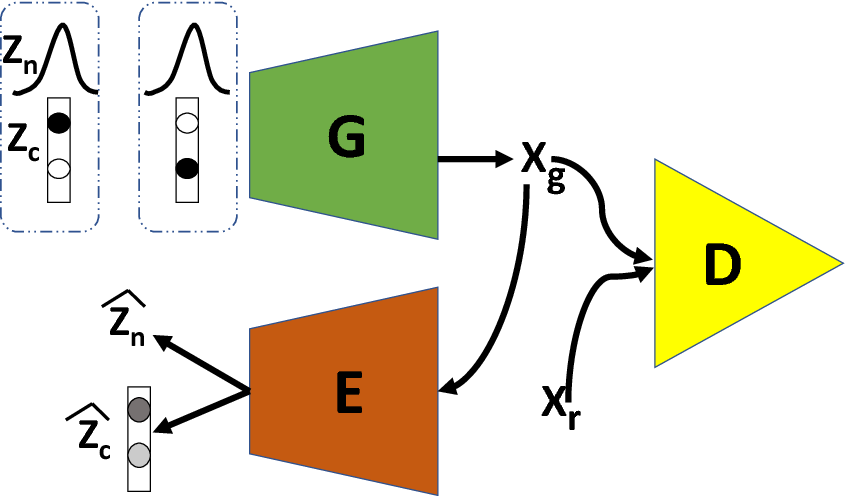
\includegraphics[width=0.55\textwidth, keepaspectratio]{./images/ClusterGAN_model.png}
% 	\begin{itemize}
% 		\item campionare casualmente variabili latenti da un mix tra vettori "one-hot" $z_c$ e valori continui $z_n$
% 		\item "dare in pasto" i valori campionati alla GAN e i dati reali $x_r$ al discriminatore
% 		\item accoppiare un encoder alla GAN che proietti i dati generati $x_g$ sullo spazio latente
% 		\item utilizzare una loss specifica per il clustering
% 	\end{itemize}
% \end{frame}

\section{Preliminary Results}

\begin{frame}{Objective Metrics for Clustering}
\begin{minipage}[0.95\textheight]{\textwidth}
\begin{columns}[T]
	\begin{column}{0.33\textwidth}
	Silhouette Score
	\centering
	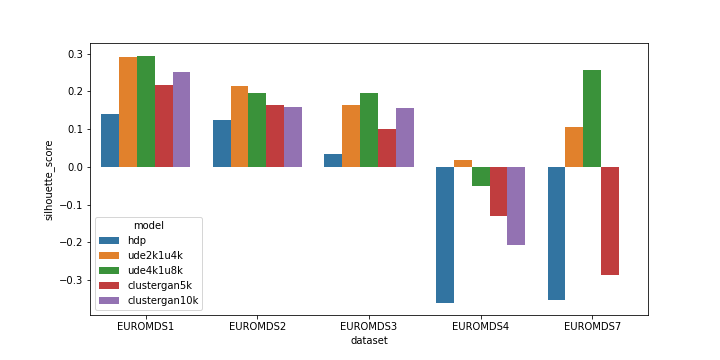
\includegraphics[width=\textwidth, keepaspectratio]{./images/silh_score.png}
	\end{column}
	\begin{column}{0.33\textwidth}
	Calinski Harabasz Score
	\centering
	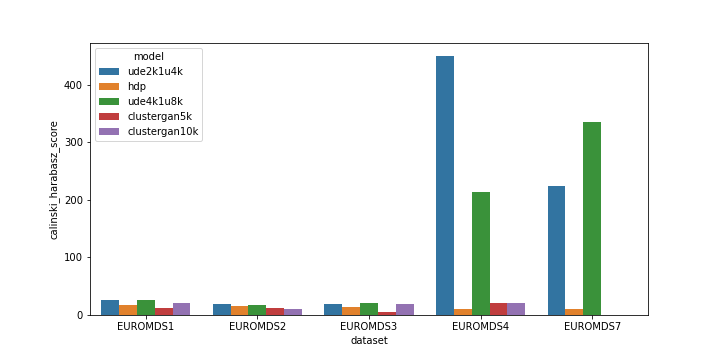
\includegraphics[width=\textwidth, keepaspectratio]{./images/cal_har_score.png}
	\end{column}
	% \begin{column}{0.33\textwidth}
	% Davies Bouldin Score
	% \centering
	% \includegraphics[width=\textwidth, keepaspectratio]{./images/dav_bou_score.png}
	% \end{column}
\end{columns}
\end{minipage}
\end{frame}

\begin{frame}{}
\end{frame}


\section{Conclusione}

\begin{frame}{Bibliografia}
	\fontsize{8pt}{7.2}\selectfont
	\bibliographystyle{plain}
	\bibliography{bibliography}
\end{frame}

\begin{frame}{}
	The End,\\
	Thanks for the attention
\end{frame}

\end{document}